\documentclass[11pt,a4paper]{article}

\usepackage[utf8]{inputenc}
\usepackage[T1]{fontenc}
\usepackage{amsmath,amssymb}
\usepackage{booktabs}
\usepackage{multirow}
\usepackage{hyperref}
\usepackage{tikz}
\usepackage[margin=2.5cm]{geometry}
\usepackage{listings}
\usepackage{xcolor}

\usetikzlibrary{trees,arrows.meta,shapes.geometric}

\lstset{
  basicstyle=\ttfamily\small,
  keywordstyle=\color{blue},
  commentstyle=\color{gray},
  breaklines=true,
  frame=single
}

\title{The \texttt{-guess} Option in CBC/CLP:\\Automatic LP Parameter Selection}
\author{Auto-generated documentation from source code analysis}
\date{March 2026}

\begin{document}
\maketitle

\begin{abstract}
The \texttt{-guess} command in CBC (and CLP) inspects structural properties
of the loaded LP model and returns a string of solver parameters predicted to
yield good performance.  This document describes the decision logic
implemented in \texttt{ClpSimplexOther::guess()}, the features it examines,
and the parameter configurations it produces.  A decision tree diagram
summarises the complete logic.
\end{abstract}

\tableofcontents

%% -----------------------------------------------------------------------
\section{Overview}

When the user issues the \texttt{guess} action inside the CBC interactive
shell (or calls it through the C interface), the following chain of events
occurs:

\begin{enumerate}
  \item The current LP model is obtained from the \texttt{OsiClpSolverInterface}.
  \item The model pointer is cast to \texttt{ClpSimplexOther}.
  \item The method \texttt{ClpSimplexOther::guess(int mode)} is called.
  \item The returned string of CLP command-line flags is injected into the
        command queue, overriding the default LP strategy for the subsequent
        solve.
\end{enumerate}

The idea is rooted in the \emph{algorithm selection} literature: different LP
instances respond better to different solver configurations, and a small set
of cheaply computable instance features can predict which configuration to
use.  The reference work underlying the feature infrastructure is:

\begin{quote}
Vilas Boas, M.\,G.; Santos, H.\,G.; Merschmann, L.\,H.\,C.\ and Vanden
Berghe, G.\ \emph{Optimal Decision Trees for the Algorithm Selection Problem:
Integer Programming Based Approaches.}  International Transactions in
Operational Research, DOI 10.1111/itor.12724, 2019.
\end{quote}

%% -----------------------------------------------------------------------
\section{Features Examined}

The \texttt{guess()} method computes three features from the model:

\begin{enumerate}
  \item \textbf{allInt} --- a Boolean flag that is \texttt{true} when every
        variable with a non-trivial bound range
        ($u_j > l_j$) is declared integer.  Continuous variables whose lower
        and upper bounds coincide (fixed variables) are ignored.
  \item \textbf{average} --- the arithmetic mean of the objective function
        coefficients:
        \[
          \text{average} = \frac{1}{n}\sum_{j=1}^{n} c_j
        \]
        where $n$ is the number of columns and $c_j$ are the (sorted)
        objective coefficients.
  \item \textbf{median} --- the median objective coefficient, taken as the
        element at position $\lfloor n/2 \rfloor$ of the sorted objective
        vector.
\end{enumerate}

These features are computed in $O(n \log n)$ time (dominated by the sort of
the objective vector).

%% -----------------------------------------------------------------------
\section{Decision Logic}

The decision tree has depth two.  The first split is on \textbf{allInt}; the
second split depends on the branch:

\begin{itemize}
  \item If \textbf{allInt} is true, the split is on
        $\text{average} \leq 0.0086207$.
  \item If \textbf{allInt} is false, the split is on
        $\text{median} \leq 0.75$.
\end{itemize}

This yields four leaf configurations, described in
Table~\ref{tab:leaves}.

\begin{table}[htbp]
\centering
\caption{Parameter configurations at each leaf of the decision tree.}
\label{tab:leaves}
\begin{tabular}{@{}llp{8cm}@{}}
\toprule
\textbf{Leaf} & \textbf{Condition} & \textbf{Parameters} \\
\midrule
L1 & allInt $\wedge$ average $\leq 0.0086207$
   & \texttt{-idiot 30 -pertvalue -1483 -primals} \\
L2 & allInt $\wedge$ average $> 0.0086207$
   & \texttt{-idiot 60 -primals} \\
L3 & $\neg$allInt $\wedge$ median $\leq 0.75$
   & \texttt{-dualpivot pesteep -psi 1.0 -pertv 52 -duals} \\
L4 & $\neg$allInt $\wedge$ median $> 0.75$
   & \texttt{-idiot 80 -primals} \\
\bottomrule
\end{tabular}
\end{table}

%% -----------------------------------------------------------------------
\section{Decision Tree Diagram}

\begin{figure}[htbp]
\centering
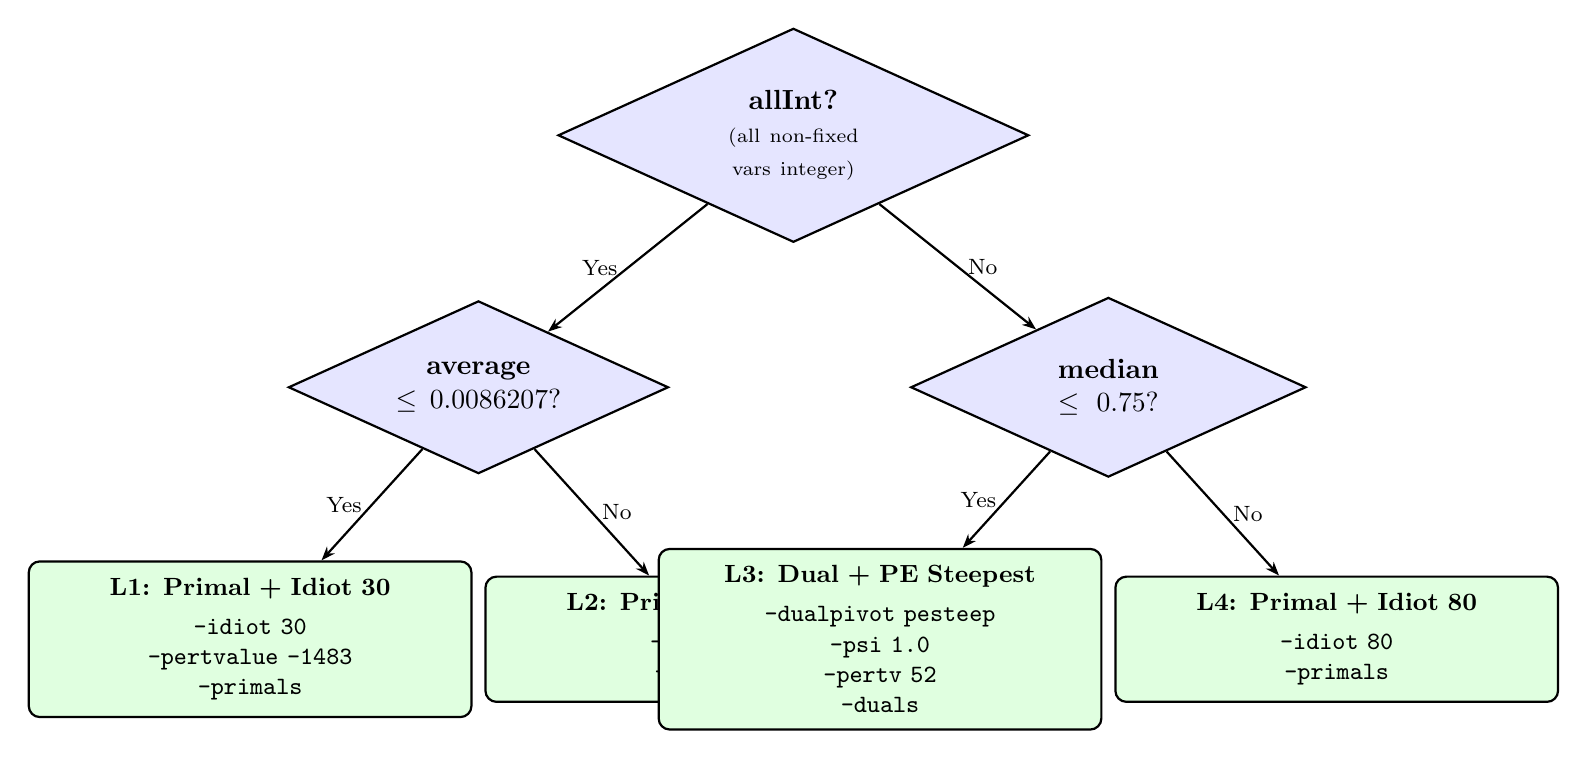
\begin{tikzpicture}[
    grow=down,
    level distance=3.2cm,
    sibling distance=7.5cm,
    every node/.style={align=center},
    decision/.style={diamond, draw, thick, inner sep=2pt,
                     fill=blue!10, text width=3cm,
                     aspect=2.2},
    leaf/.style={rectangle, draw, thick, rounded corners,
                 fill=green!12, text width=5.2cm,
                 inner sep=6pt, font=\small},
    edge from parent/.style={draw, thick, -{Stealth[length=5pt]}},
    level 1/.style={sibling distance=8cm},
    level 2/.style={sibling distance=5.8cm},
]

\node [decision] {\textbf{allInt?}\\{\scriptsize(all non-fixed vars integer)}}
  child {
    node [decision] {\textbf{average}\\$\leq 0.0086207$?}
    child {
      node [leaf] {\textbf{L1: Primal + Idiot 30}\\[3pt]
        \texttt{-idiot 30}\\
        \texttt{-pertvalue -1483}\\
        \texttt{-primals}}
      edge from parent node[left, font=\footnotesize] {Yes}
    }
    child {
      node [leaf] {\textbf{L2: Primal + Idiot 60}\\[3pt]
        \texttt{-idiot 60}\\
        \texttt{-primals}}
      edge from parent node[right, font=\footnotesize] {No}
    }
    edge from parent node[left, font=\footnotesize] {Yes}
  }
  child {
    node [decision] {\textbf{median}\\$\leq 0.75$?}
    child {
      node [leaf] {\textbf{L3: Dual + PE Steepest}\\[3pt]
        \texttt{-dualpivot pesteep}\\
        \texttt{-psi 1.0}\\
        \texttt{-pertv 52}\\
        \texttt{-duals}}
      edge from parent node[left, font=\footnotesize] {Yes}
    }
    child {
      node [leaf] {\textbf{L4: Primal + Idiot 80}\\[3pt]
        \texttt{-idiot 80}\\
        \texttt{-primals}}
      edge from parent node[right, font=\footnotesize] {No}
    }
    edge from parent node[right, font=\footnotesize] {No}
  };

\end{tikzpicture}
\caption{Decision tree implemented by \texttt{ClpSimplexOther::guess()}.}
\label{fig:tree}
\end{figure}

%% -----------------------------------------------------------------------
\section{Parameter Descriptions}

\subsection{LP Algorithm Selection}

\begin{description}
  \item[\texttt{-primals}] Solve the LP relaxation using the primal simplex
    method.  Chosen in three of the four leaves (L1, L2, L4).
  \item[\texttt{-duals}] Solve the LP relaxation using the dual simplex
    method.  Chosen only in leaf L3.
\end{description}

\subsection{Idiot Crash}

\begin{description}
  \item[\texttt{-idiot $k$}] Run $k$ iterations of the ``idiot'' crash
    procedure before starting simplex.  The idiot crash is a
    Lagrangian-relaxation-based heuristic that produces a warm-start basis
    for the primal simplex.  Higher values invest more effort in the crash
    phase.  The tree selects 30, 60, or 80 iterations depending on the
    model class.
\end{description}

\subsection{Perturbation}

\begin{description}
  \item[\texttt{-pertvalue $v$}] Sets the perturbation value used to break
    degeneracy.  A negative value (here $-1483$) triggers a specific
    internal perturbation strategy in CLP.  Used only in leaf L1.
  \item[\texttt{-pertv $v$}] Sets the perturbation value for the dual
    simplex (here $52$).  Used only in leaf L3.
\end{description}

\subsection{Dual Pivot Strategy}

\begin{description}
  \item[\texttt{-dualpivot pesteep}] Use the Positive Edge steepest-edge
    dual pivot rule.  This is a variant of the steepest-edge pivot that
    incorporates the positive edge criterion to improve dual simplex
    performance.  Used only in leaf L3.
  \item[\texttt{-psi $\psi$}] The $\psi$ parameter controls the weight
    given to the positive-edge criterion in the dual pivot selection.
    A value of $1.0$ gives full weight to the positive-edge component.
    Used only in leaf L3.
\end{description}

%% -----------------------------------------------------------------------
\section{Integration in CBC}

The \texttt{guess} action is registered as a CLP parameter
(\texttt{ClpParam::GUESS}).  When triggered from the CBC shell, the code in
\texttt{CbcSolver.cpp} performs:

\begin{lstlisting}[language=C++]
ClpSimplexOther *model2 =
    static_cast<ClpSimplexOther *>(lpSolver);
std::string input = model2->guess(0);
// inject into command queue
\end{lstlisting}

The returned string (e.g.\ \texttt{"-idiot 60 -primals"}) is parsed and
pushed onto the input command queue, so the subsequent LP solve uses the
recommended settings.

In the C~interface (\texttt{Cbc\_C\_Interface.cpp}), the same logic is
invoked when the LP method is set to \texttt{LPM\_Auto}.  The returned
string is parsed to extract individual parameters (idiot passes,
perturbation value, $\psi$, dual pivot strategy, and LP method) which are
then stored in the model's parameter arrays.

%% -----------------------------------------------------------------------
\section{Broader Context: OsiFeatures}

While the current \texttt{guess()} implementation uses only three simple
features (allInt, average objective, median objective), the CBC/Osi
infrastructure includes a much richer feature extraction framework in
\texttt{OsiFeatures} (207~features), covering:

\begin{itemize}
  \item Problem dimensions (rows, columns, density, non-zeros).
  \item Variable types (binary, general integer, continuous, unbounded).
  \item Constraint classification (partitioning, packing, covering,
        cardinality, knapsack, bin-packing, flow, singleton, aggregation,
        precedence, variable bound, mixed-binary, general integer).
  \item Coefficient matrix statistics (min, max, mean, std.\ dev., ratio
        of largest to smallest absolute value, integrality).
  \item Objective function and RHS statistics.
  \item Row and column non-zero distribution histograms.
\end{itemize}

These features are used by the \texttt{CbcInstanceFeatures} class to write
CSV files for offline algorithm selection studies.  A natural extension would
be to replace the hand-crafted decision tree in \texttt{guess()} with a
learned model trained on these 207~features.

%% -----------------------------------------------------------------------
\section{Source Code Locations}

\begin{table}[htbp]
\centering
\begin{tabular}{@{}lp{8cm}@{}}
\toprule
\textbf{File} & \textbf{Role} \\
\midrule
\texttt{Clp/src/ClpSimplexOther.cpp} (line $\sim$11037) &
  Implementation of \texttt{guess()} \\
\texttt{Cbc/src/CbcSolver.cpp} (line $\sim$3613) &
  Invocation from CBC shell \\
\texttt{Cbc/src/Cbc\_C\_Interface.cpp} (line $\sim$1879) &
  Invocation from C interface \\
\texttt{Osi/src/Osi/OsiFeatures.hpp} &
  Full feature enumeration (207 features) \\
\texttt{Osi/src/Osi/OsiFeatures.cpp} &
  Feature computation \\
\texttt{Cbc/src/CbcInstanceFeatures.cpp} &
  CSV export of features \\
\bottomrule
\end{tabular}
\end{table}

%% -----------------------------------------------------------------------
\section{Absence of Barrier and Future Extensions}

\subsection{Barrier Is Never Selected}

The current \texttt{guess()} implementation never returns a barrier
(interior point) configuration.  All four leaves select either primal or
dual simplex.  The C~interface parsing code in
\texttt{Cbc\_C\_Interface.cpp} does check for \texttt{"-barrier"} in the
returned string, but this branch is currently dead code---it was written in
anticipation of a future extension.

\subsection{When Barrier Would Be Appropriate}

Barrier methods tend to outperform simplex on LP relaxations that exhibit
one or more of the following characteristics:

\begin{itemize}
  \item \textbf{Large and dense} constraint matrices (high non-zeros per
        row/column).
  \item \textbf{Highly degenerate} problems where simplex stalls due to
        many variables at bounds.
  \item \textbf{Network or flow structure} that yields favourable Cholesky
        factorisation sparsity.
  \item \textbf{High proportion of equalities}, which produce
        better-conditioned normal equations for the barrier method while
        causing degeneracy issues for dual simplex.
\end{itemize}

A useful heuristic filter on the OsiFeatures to identify barrier-friendly
instances is:
\[
  \texttt{OFdensity} > 1.0\%, \quad
  \texttt{OFrowNzAvg} > 50, \quad
  \texttt{OFrows} > 5000, \quad
  \texttt{OFpercEqualities} > 40\%.
\]

\subsection{Candidate MIPLIB 2017 Instances for Barrier Experiments}

Table~\ref{tab:barrier} lists MIPLIB 2017 instances whose LP relaxations
have structural properties that suggest barrier may be competitive or
superior to simplex.

\begin{table}[htbp]
\centering
\caption{MIPLIB 2017 instances likely to benefit from barrier for the LP relaxation.}
\label{tab:barrier}
\begin{tabular}{@{}llp{6.5cm}@{}}
\toprule
\textbf{Category} & \textbf{Instance} & \textbf{Rationale} \\
\midrule
\multirow{4}{*}{Dense / large-scale}
  & \texttt{neos-5075914-elvire}  & Large, dense constraint matrix \\
  & \texttt{neos-3083819-nubia}   & High density, many nz per row \\
  & \texttt{supportcase18}        & Large-scale, dense blocks \\
  & \texttt{graph40-80-1rand}     & Dense graph-based structure \\
\midrule
\multirow{4}{*}{Network / flow}
  & \texttt{mc11}                 & Multicommodity flow \\
  & \texttt{momentum1}            & Large network structure \\
  & \texttt{neos-4954672-berkel}  & Flow-like, many equalities \\
  & \texttt{supportcase6}         & Large flow/network relaxation \\
\midrule
\multirow{3}{*}{Highly degenerate}
  & \texttt{neos-3627168-kasai}   & Degenerate LP, simplex stalls \\
  & \texttt{neos-4338804-snowy}   & Degenerate, simplex struggles \\
  & \texttt{seymour}              & Classic difficult degenerate LP \\
\bottomrule
\end{tabular}
\end{table}

\subsection{Proposed Training Pipeline for an Improved Decision Tree}
\label{sec:pipeline}

The infrastructure for a learned replacement of the hand-crafted tree is
largely in place.  The following pipeline is proposed:

\begin{enumerate}
  \item \textbf{Feature extraction.}  Use
        \texttt{CbcInstanceFeatures::extract()} and
        \texttt{writeCsv()} on a large benchmark set (MIPLIB~2017,
        Mittelmann, Netlib) to obtain the 207 OsiFeatures per instance.
  \item \textbf{Configuration space.}  Define the candidate LP
        configurations, including at minimum the current four leaves plus
        barrier:
        \begin{itemize}
          \item \texttt{-idiot 30 -pertvalue -1483 -primals}
          \item \texttt{-idiot 60 -primals}
          \item \texttt{-dualpivot pesteep -psi 1.0 -pertv 52 -duals}
          \item \texttt{-idiot 80 -primals}
          \item \texttt{-barrier}
        \end{itemize}
  \item \textbf{Benchmark.}  Solve each instance's LP relaxation with
        every candidate configuration.  Record wall-clock time.
  \item \textbf{Labelling.}  For each instance, assign the label of the
        fastest configuration.
  \item \textbf{Tree training.}  Train an optimal decision tree using one
        of the methods in Table~\ref{tab:tree-methods}.
  \item \textbf{Code generation.}  Convert the learned tree into a C++
        \texttt{if/else} block and replace the body of
        \texttt{ClpSimplexOther::guess()}.
\end{enumerate}

\begin{table}[htbp]
\centering
\caption{Decision tree training methods suitable for embedding in C++.}
\label{tab:tree-methods}
\begin{tabular}{@{}lp{9cm}@{}}
\toprule
\textbf{Method} & \textbf{Notes} \\
\midrule
CART (greedy) & Simple, fast to train; may be suboptimal for small depth budgets. \\
Optimal Classification Trees (OCT) & IP-based method from Vilas Boas et al.\ (2019); provably optimal for a given depth. \\
GOSDT & Near-optimal sparse trees; good balance of optimality and scalability. \\
\bottomrule
\end{tabular}
\end{table}

The key advantage of decision trees over other model families (random
forests, gradient boosting, neural networks) is that they compile to pure
\texttt{if/else} C++ with zero runtime dependencies---matching the
self-contained nature of the CLP/CBC codebase.

\end{document}
